% Yale University Poster - Gemini Theme
% Serial Dilution Ecological Modeling Project

\documentclass[final]{beamer}

% ====================
% Packages
% ====================

\usepackage[T1]{fontenc}
\usepackage{lmodern}
\usepackage[size=custom, width=122, height=91, scale=1.2]{beamerposter}
\usetheme{gemini}
\usecolortheme{msu}
\usepackage{graphicx}
\usepackage{booktabs}
\usepackage{tikz}
\usepackage{pgfplots}
\pgfplotsset{compat=1.14}
\usepackage{anyfontsize}
\usepackage{amsmath}
\usepackage{amssymb}
\usepackage{bm}
\usefonttheme{professionalfonts}
\renewcommand*{\normalsize}{\fontsize{30.5}{36.6}\selectfont}
\setbeamerfont{block body}{size=\normalsize}

% ====================
% Lengths
% ====================

% (3 columns) + 4 separators = paperwidth
% 4 * 0.025 + 3 * 0.30 = 0.10 + 0.90 = 1.00
\newlength{\sepwidth}
\newlength{\colwidth}
\setlength{\sepwidth}{0.025\paperwidth}
\setlength{\colwidth}{0.30\paperwidth}

\newcommand{\separatorcolumn}{\begin{column}{\sepwidth}\end{column}}

% ====================
% Title & Authors
% ====================

\title{Low-Dimensional Microbial Assembly: A Latent Consumer-Resource Neural ODE for Serial Dilution Ecology}

\author{Karthik Srinivasan\textsuperscript{1}, Germ\'an Plata\textsuperscript{2}, Purushottam Dixit\textsuperscript{1}}

\institute[shortinst]{\textsuperscript{1}Department of Biomedical Engineering, Yale University \samelineand \textsuperscript{2}Computational Sciences, BiomEdit, LLC.}

% ====================
% Footer & Logos
% ====================

\footercontent{
  \textbf{Cross-Dataset Benchmarks:} Venturelli et al. (\textit{Mol. Syst. Biol.} 2018) \;\textbullet\; Jin et al. (\textit{Nat. Commun.} 2023) \;\textbullet\; German et al. (BiomEdit Inc., Virginia Tech) \;\textbullet\; Hu et al. (\textit{Science} 2022)
  \hfill
  \href{mailto:karthik.srinivasan@yale.edu}{karthik.srinivasan@yale.edu}
}

\logoleft{
\includegraphics[height=5.2cm]{logos/logo.png}}
\logoright{
\includegraphics[height=4.6cm]{figures/attribution_and_qr.png}\hspace{3.0cm}\mbox{}}

% ====================
% Document Body
% ====================

\begin{document}

\begin{frame}[t]
\begin{columns}[t]
\separatorcolumn

% ════════════════════════════════════════════════════════════════════════════════
% COLUMN 1: Foundations & Out-of-Sample Generalization (Ophelia)
% ════════════════════════════════════════════════════════════════════════════════
\begin{column}{\colwidth}

  % 1. SERIAL DILUTION ECOLOGY
  \begin{block}{Serial dilution is a controlled, repeatable ecology experiment}
    \begin{minipage}[c]{0.64\linewidth}
      \begin{itemize}
        \item Grow microbes in batches, then transfer a measured fraction into fresh medium to begin the next cycle.
        \vspace{20pt}
        \item Control community composition, nutrients, dilution, and growth conditions to systematically test ecological theories.
        \vspace{20pt}
        \item Models help navigate the many possible combinations of these variables to design communities, prioritize informative experiments, and generate testable predictions.
      \end{itemize}
    \end{minipage}\hfill
    \begin{minipage}[c]{0.32\linewidth}
      \centering
      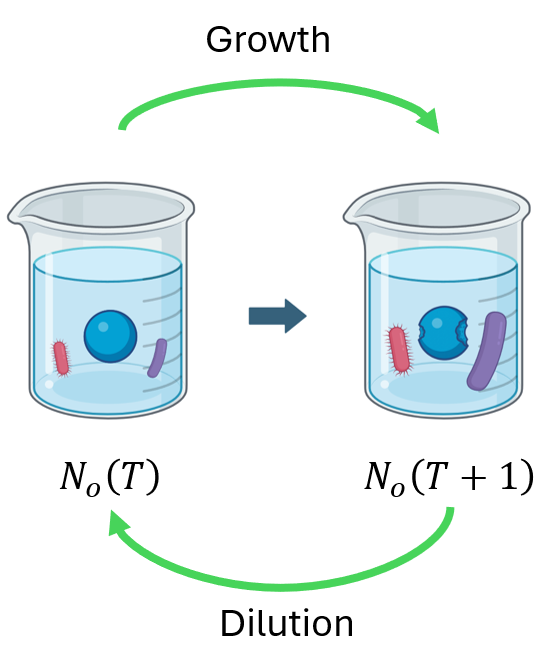
\includegraphics[width=\linewidth]{Serial dilution.png}
    \end{minipage}
  \end{block}

  % 2. BACKGROUND & DILEMMA
  \begin{block}{Current models fail to extrapolate dynamics of serial dilution}
    \begin{itemize}
      \item \textbf{Consumer-resource models:} Mechanistic and interpretable, but their many species--resource parameters make fitting raw abundance data difficult.
      \item \textbf{Machine-learning models:} Can fit abundance data, but often lack interpretable mechanisms and fail to generalize to unseen environments or bacteria.
      \item \textbf{gLV models:} A quasi-mechanistic middle ground, but also hard to fit to data due to excessive parameters ($N^2$ pairwise interactions) that are condition-specific and largely latent.
    \end{itemize}
    \begin{figure}
      \centering
      \begin{minipage}[t]{0.32\linewidth}
        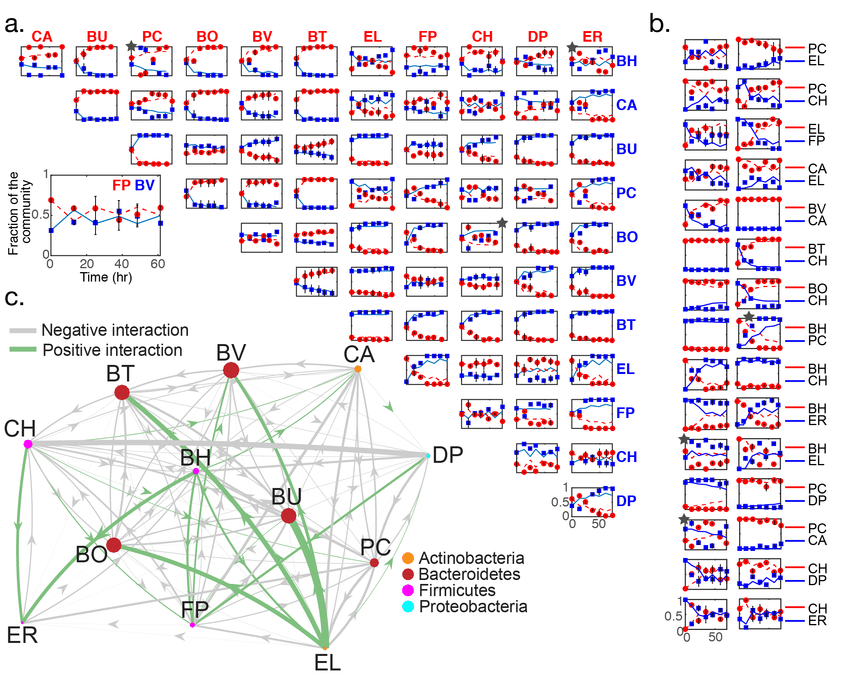
\includegraphics[height=11cm, width=\linewidth, keepaspectratio]{gLV_image.png}
        \par\vspace{6pt}{\scriptsize\textit{gLVs - Venturelli et al.\ (MSB 2018)}}
      \end{minipage}\hfill
      \begin{minipage}[t]{0.32\linewidth}
        \centering
        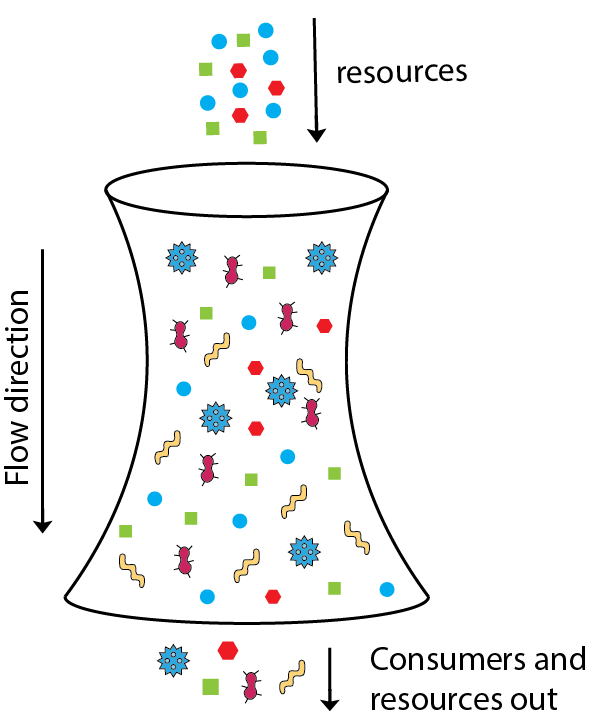
\includegraphics[height=11cm, width=\linewidth, keepaspectratio]{CRM.png}
        \par\vspace{6pt}{\scriptsize\textit{Consumer-resource models}}
      \end{minipage}\hfill
      \begin{minipage}[t]{0.32\linewidth}
        \centering
        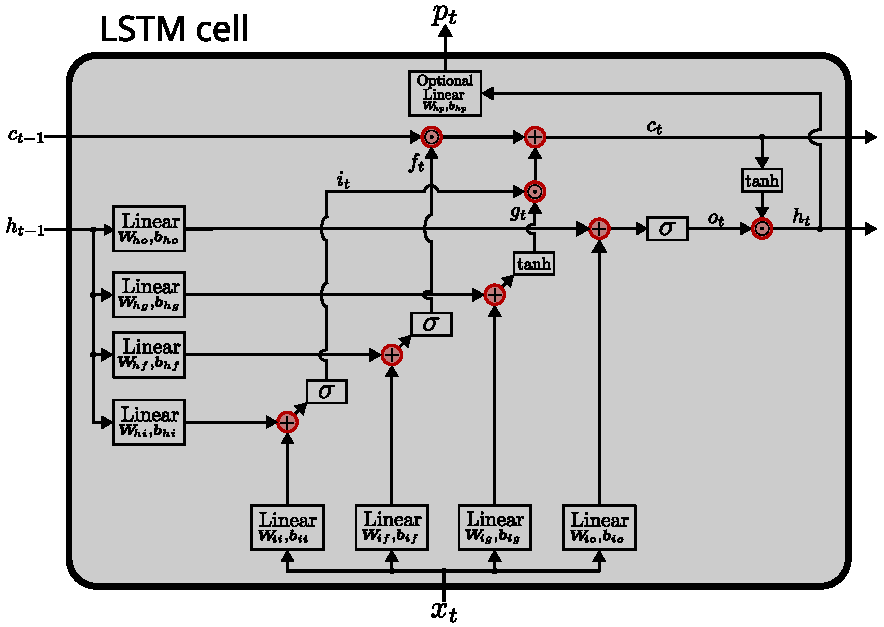
\includegraphics[height=11cm, width=\linewidth, keepaspectratio]{NN_LSTM-Cell_v2.pdf}
        \par\vspace{6pt}{\scriptsize\textit{LSTMs}}
      \end{minipage}
    \end{figure}
  \end{block}

  % 3. PHYSICAL NEURAL ODE FORMULATION
  \begin{block}{We develop a low-dimensional consumer-resource model}
    \begin{itemize}
      \item Serial-dilution communities occupy a low-dimensional niche space ($K \ll N$; Srinivasan et al., \textit{PRX Life} 2026); we represent $N$ species using $K$ latent resources.
      \vspace{10pt}
      \item Intra-passage dynamics are governed by non-equilibrium consumer-resource kinetics:
      \vspace{10pt}
      \begin{align*}
          \frac{dN_i}{dt} &= N_i \sum_k \Theta_{ik} \frac{R_k}{R_k + K_{m,k}} - \alpha_i N_i^2 \\
          \frac{dR_k}{dt} &= - \sum_i N_i \Phi_{ik} \frac{R_k}{R_k + K_{m,k}} + \sum_l W_{lk} \sum_j N_j \Phi_{jl} \frac{R_l}{R_l + K_{m,l}}
      \end{align*}
      \vspace{10pt}
      where $\bm{N}$ is species abundance, $\bm{R}$ latent resource concentration, $\bm{\Theta}$ biomass yield, $\bm{\Phi}$ resource uptake rate, and $\mathbf{W}$ metabolic cross-feeding.
      \vspace{10pt}
      \item Nonnegative yields, uptake, and cross-feeding, with $\alpha_i, K_{m,k}>0$ and $\sum_k W_{jk}<1$, enforce physical constraints and mass conservation.
      \vspace{10pt}
      \item At each transfer, biomass is diluted and migration added; the medium resets: $N_i^{(m+1)}(0)=N_i^{(m)}(\tau)/D+\mu M_{c,i}$, $R_k^{(m+1)}(0)=R_{0,c,k}$.
      \vspace{10pt}
      \item Models are trained end-to-end via scheduled teacher forcing, annealing from observed transfer inocula to fully autonomous multi-passage rollouts to stabilize stiff ODE integration and eliminate compounding drift.
    \end{itemize}
  \end{block}

  \end{column}

\separatorcolumn

% ════════════════════════════════════════════════════════════════════════════════
% COLUMN 2: Universality (Pollard) & Environmental Specificity (German)
% ════════════════════════════════════════════════════════════════════════════════
\begin{column}{\colwidth}

  % 4. HELD-OUT GENERALIZATION: OPHELIA
  \begin{block}{Model accurately predicts trajectories in unseen communities}
    \begin{itemize}
      \item Synthetic human gut communities assembled from 12 prevalent bacterial isolates grown anaerobically across monoculture, co-culture, and multi-species dropout designs.
      \item Longitudinal biomass time-series tracking species optical densities across sequential sampling intervals ($t = 12\,\text{h} \to 60\,\text{h}$) throughout batch growth cycles.
      \item Invariant consumer-resource parameters learned from training sub-communities enable continuous dynamic trajectory forecasting on completely held-out community compositions.
    \end{itemize}

    \begin{figure}
      \centering
      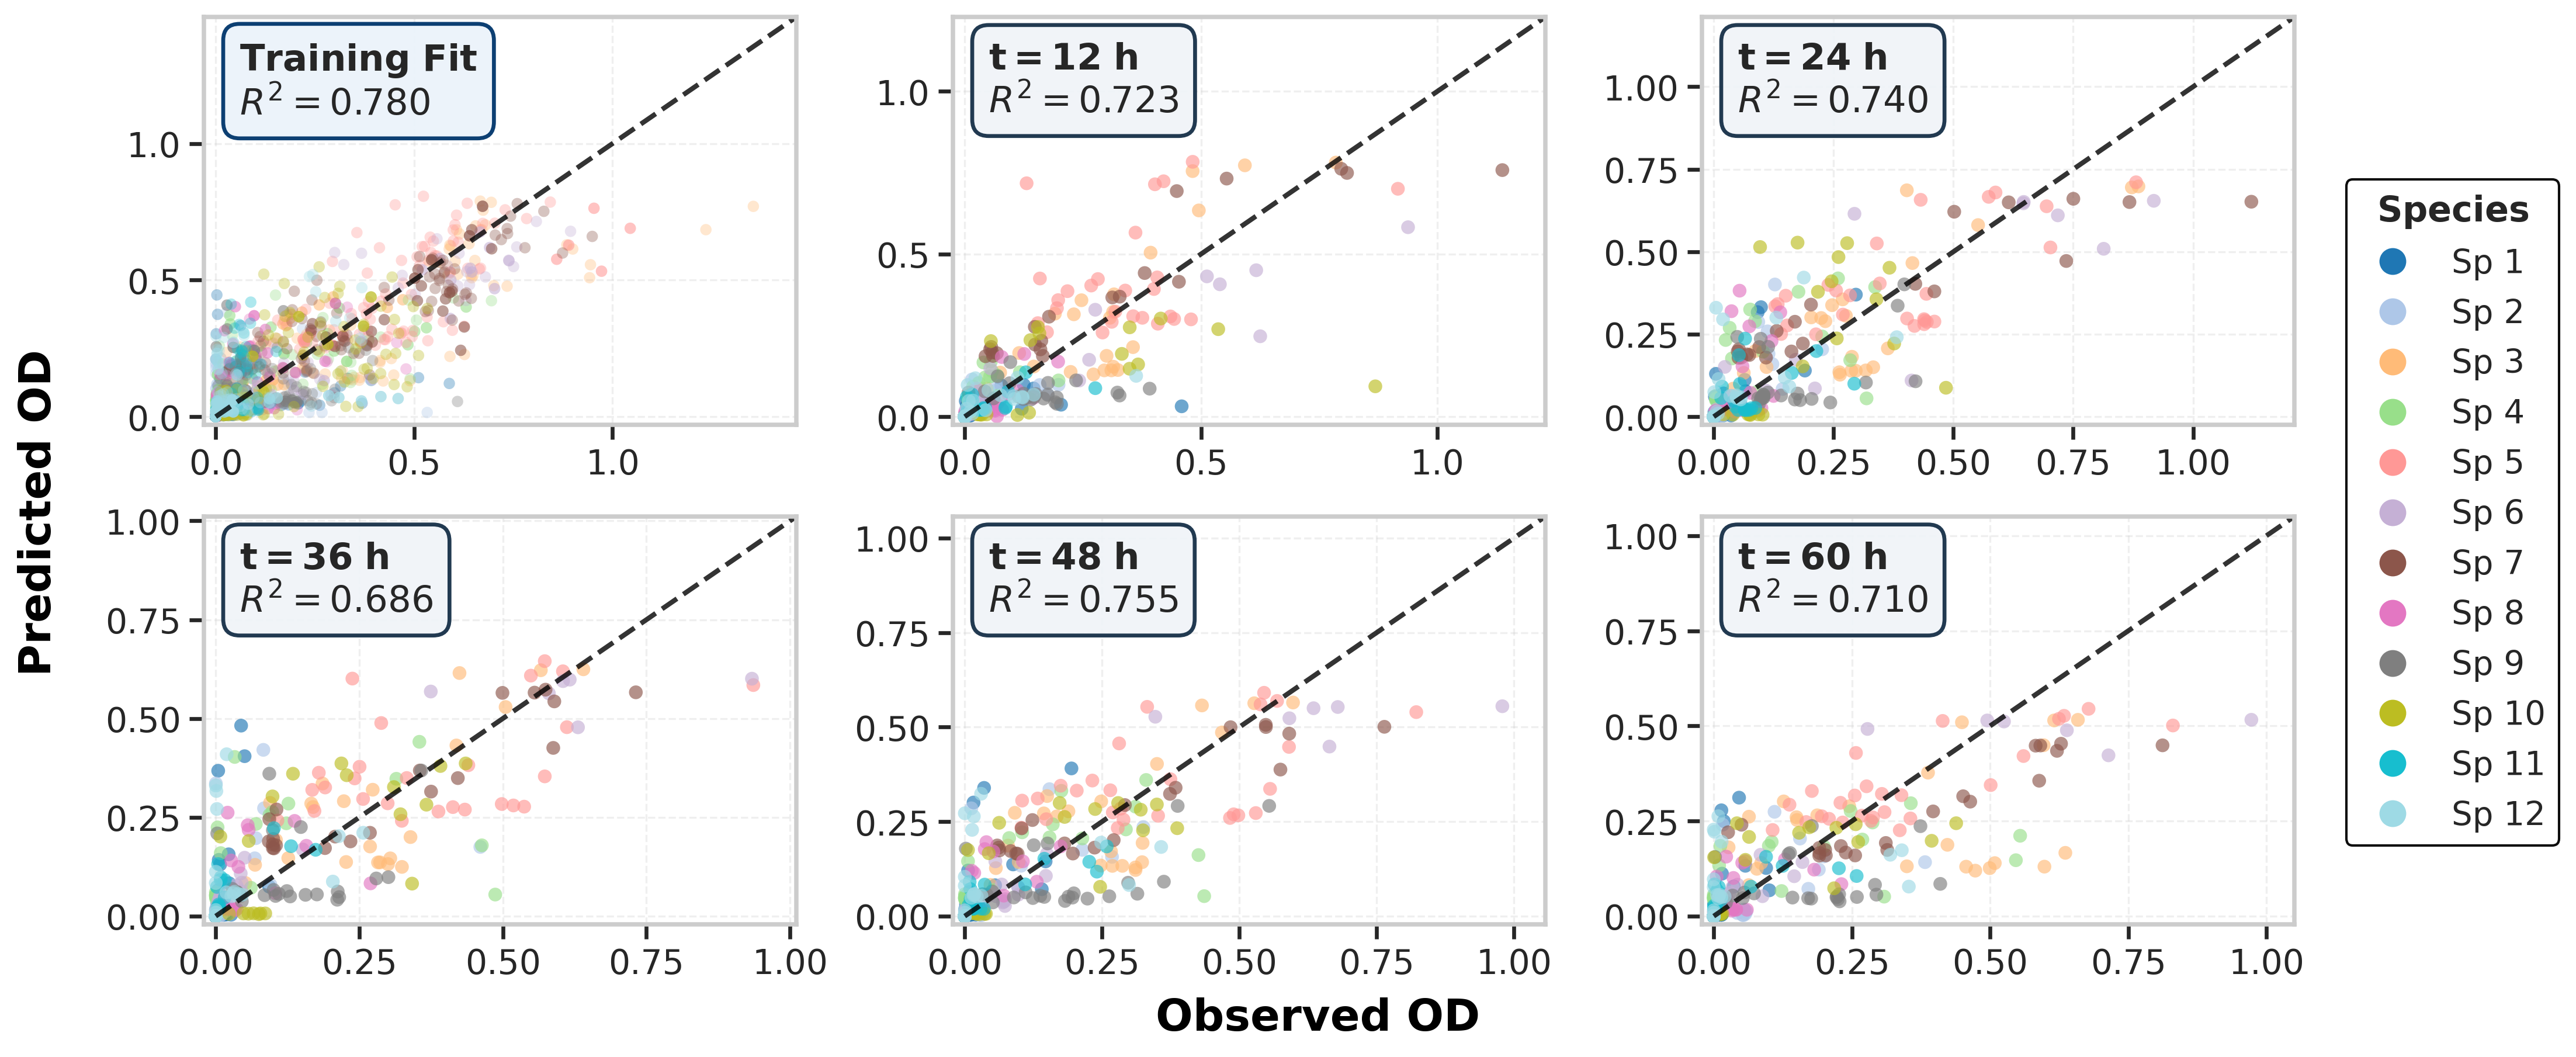
\includegraphics[width=1\linewidth]{figures/Ophelia_Test_Scatter.png}
    \end{figure}
  \end{block}



  % 5. UNIVERSALITY: POLLARD
  \begin{block}{Parameters of the model are interpretable}
    \begin{itemize}
      \item Human gut communities of 50 diverse isolates propagated through 100 serial dilution cycles across 5 spatial environments, including liquid broth and structured hydrogel beads.
      \item Multi-passage abundance profiles tracking community succession, spatial sheltering of slow-growing taxa, and long-term taxonomic retention.
      \item Invariant uptake traits $\mathbf{\Theta}$ and cross-feeding networks $\mathbf{W}$ generalize across well-mixed and structured phases without phase-specific parameter re-tuning.
    \end{itemize}

    \begin{figure}
      \centering
      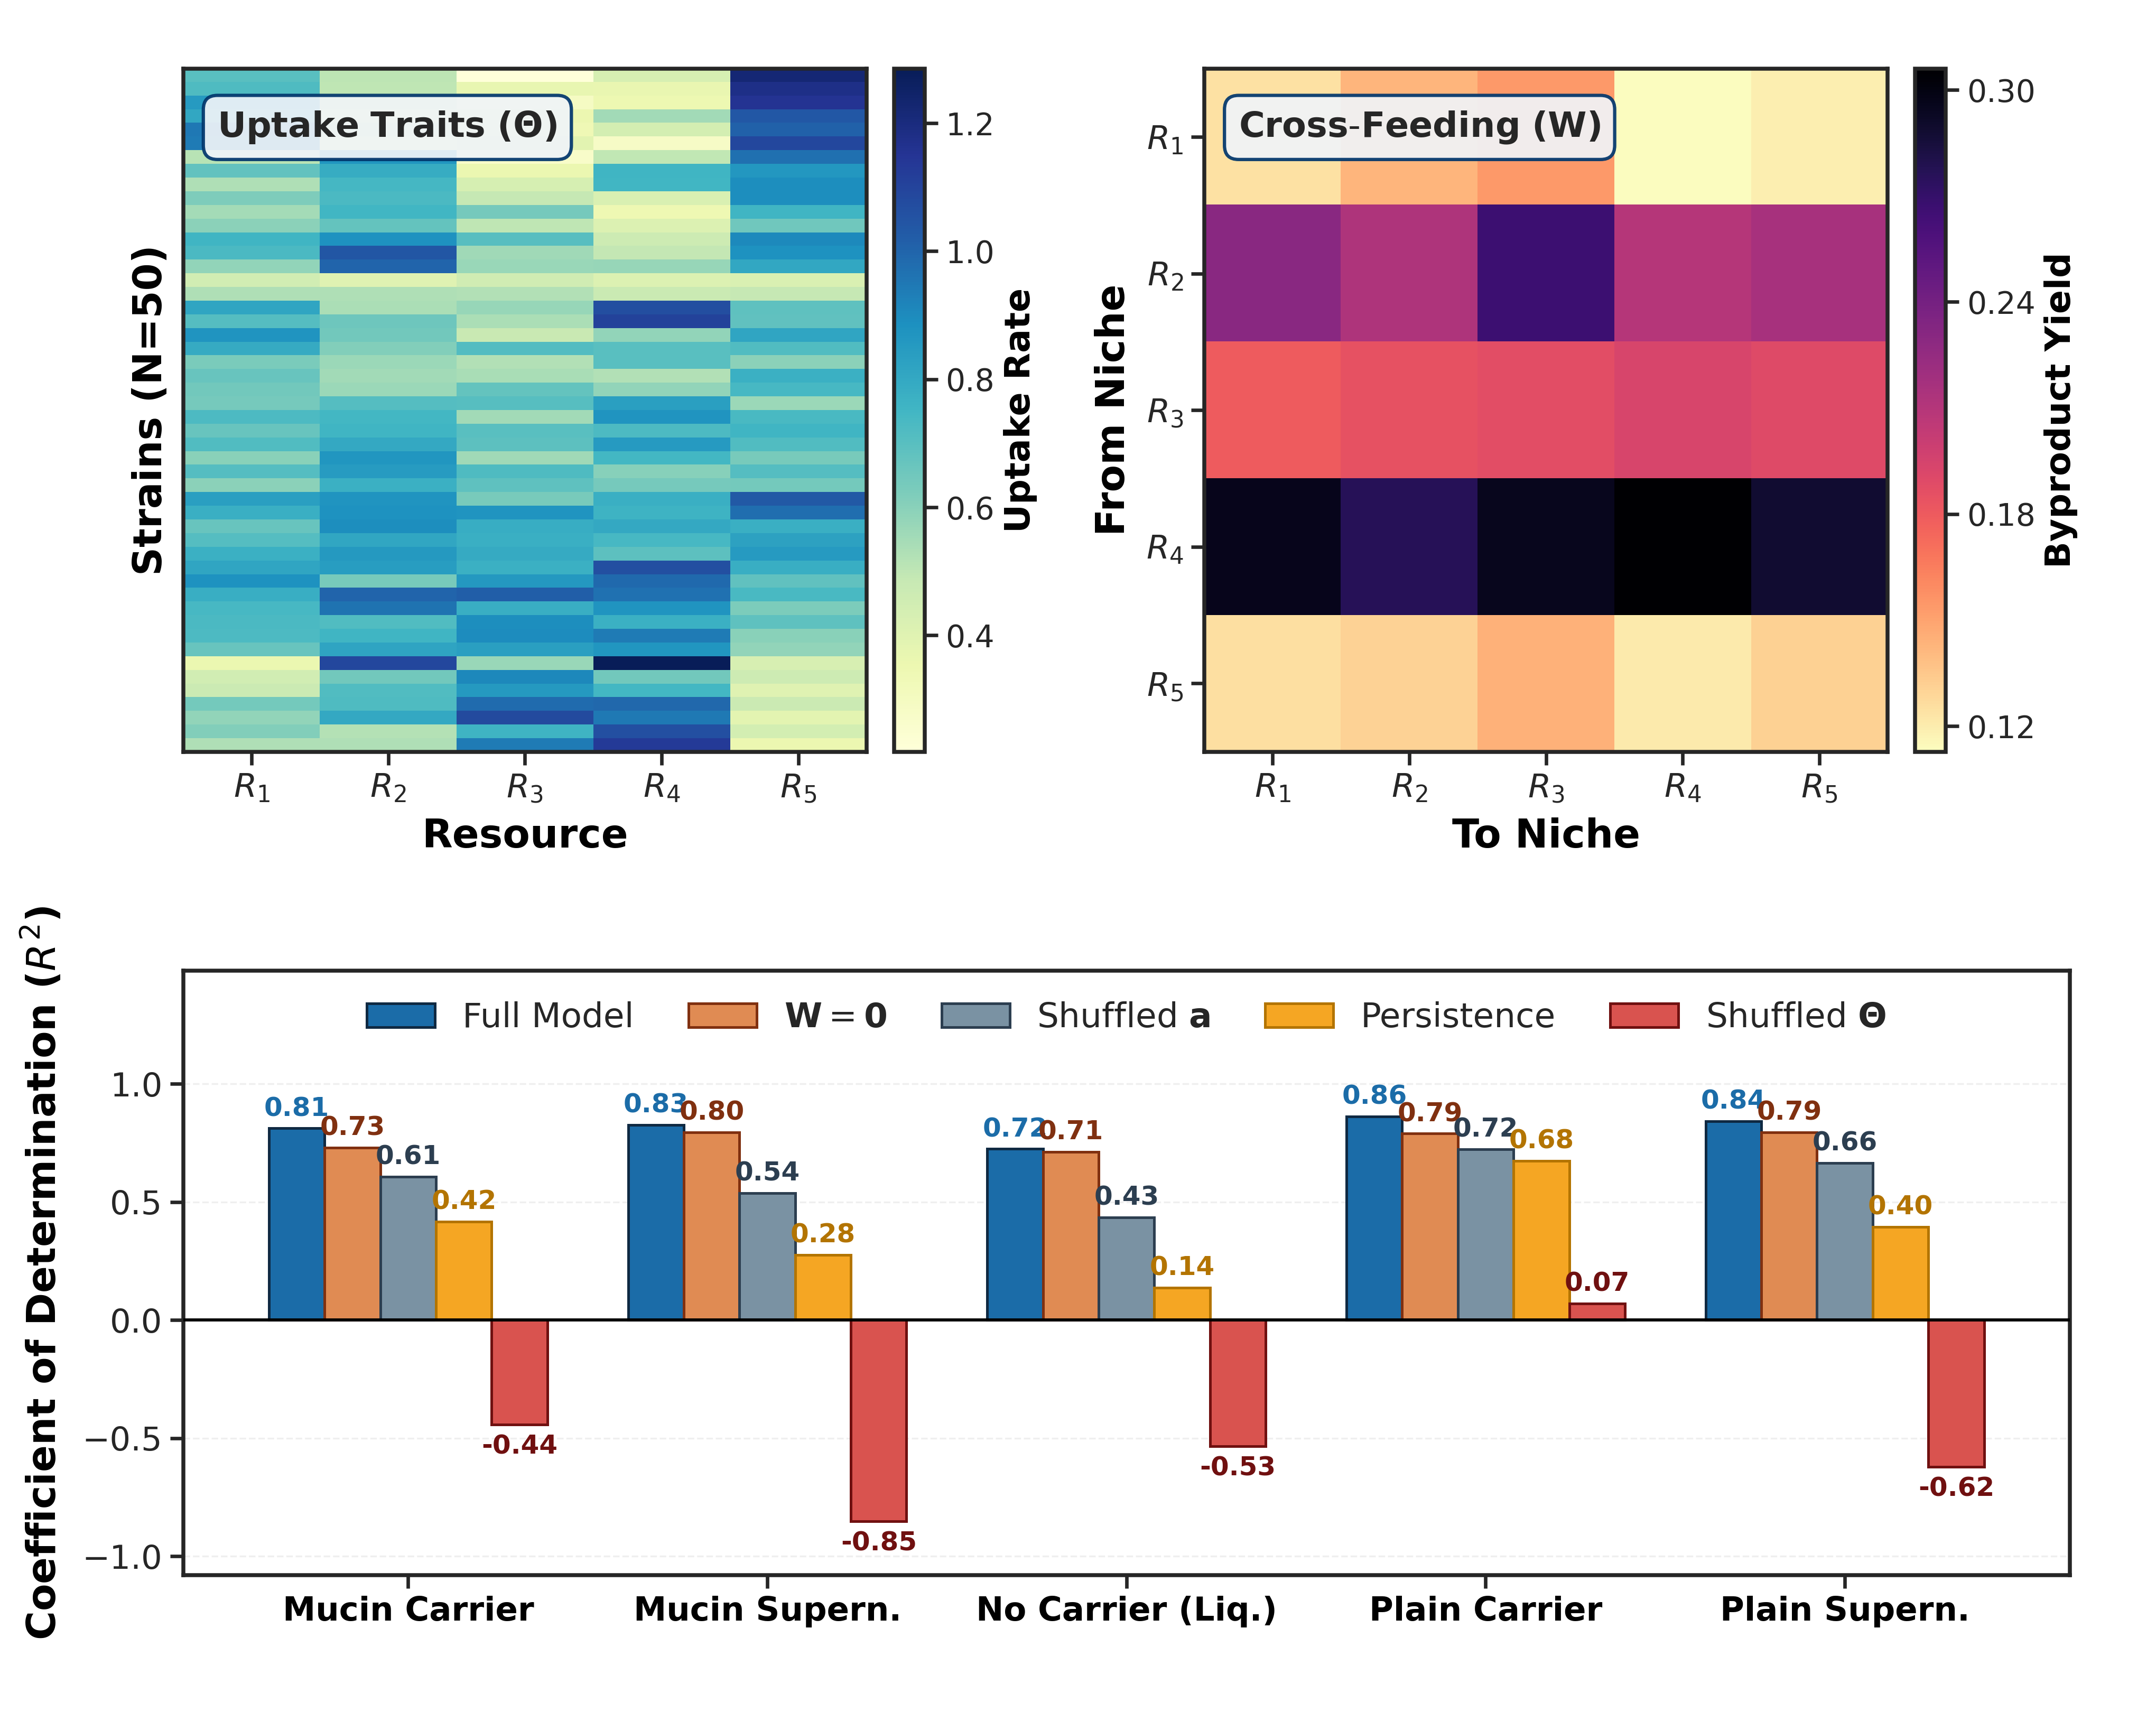
\includegraphics[width=0.96\linewidth]{figures/Pollard_Universal_Matrices.png}
    \end{figure}
  \end{block}

  \end{column}

\separatorcolumn

% ════════════════════════════════════════════════════════════════════════════════
% COLUMN 3: Phase Dynamics, Resource Trajectories & Model Extremes (Gore)
% ════════════════════════════════════════════════════════════════════════════════
\begin{column}{\colwidth}

  % 6. PREDICTIVE MEDIA SEARCH: GERMAN
  \begin{block}{Model prescribes therapeutic interventions}
    \begin{itemize}
      \item Bovine rumen inocula from distinct donors (BRRS and OSU) cultivated in pressurized bioreactors under $\mathrm{H_2:CO_2}$ (5 bar and 30 bar) with MeOH or TMA.
      \item Trained on all OSU conditions and 30 bar BRRS data; predicted 5 bar BRRS regimes to evaluate cross-donor and cross-pressure generalization.
      \item Naive cross-host therapeutic intervention fails to enrich the target microbe; our model predicts +TMA at 5 bar rescues enrichment, confirmed in wet-lab validation (23\% observed).
    \end{itemize}

    \begin{figure}
      \centering
      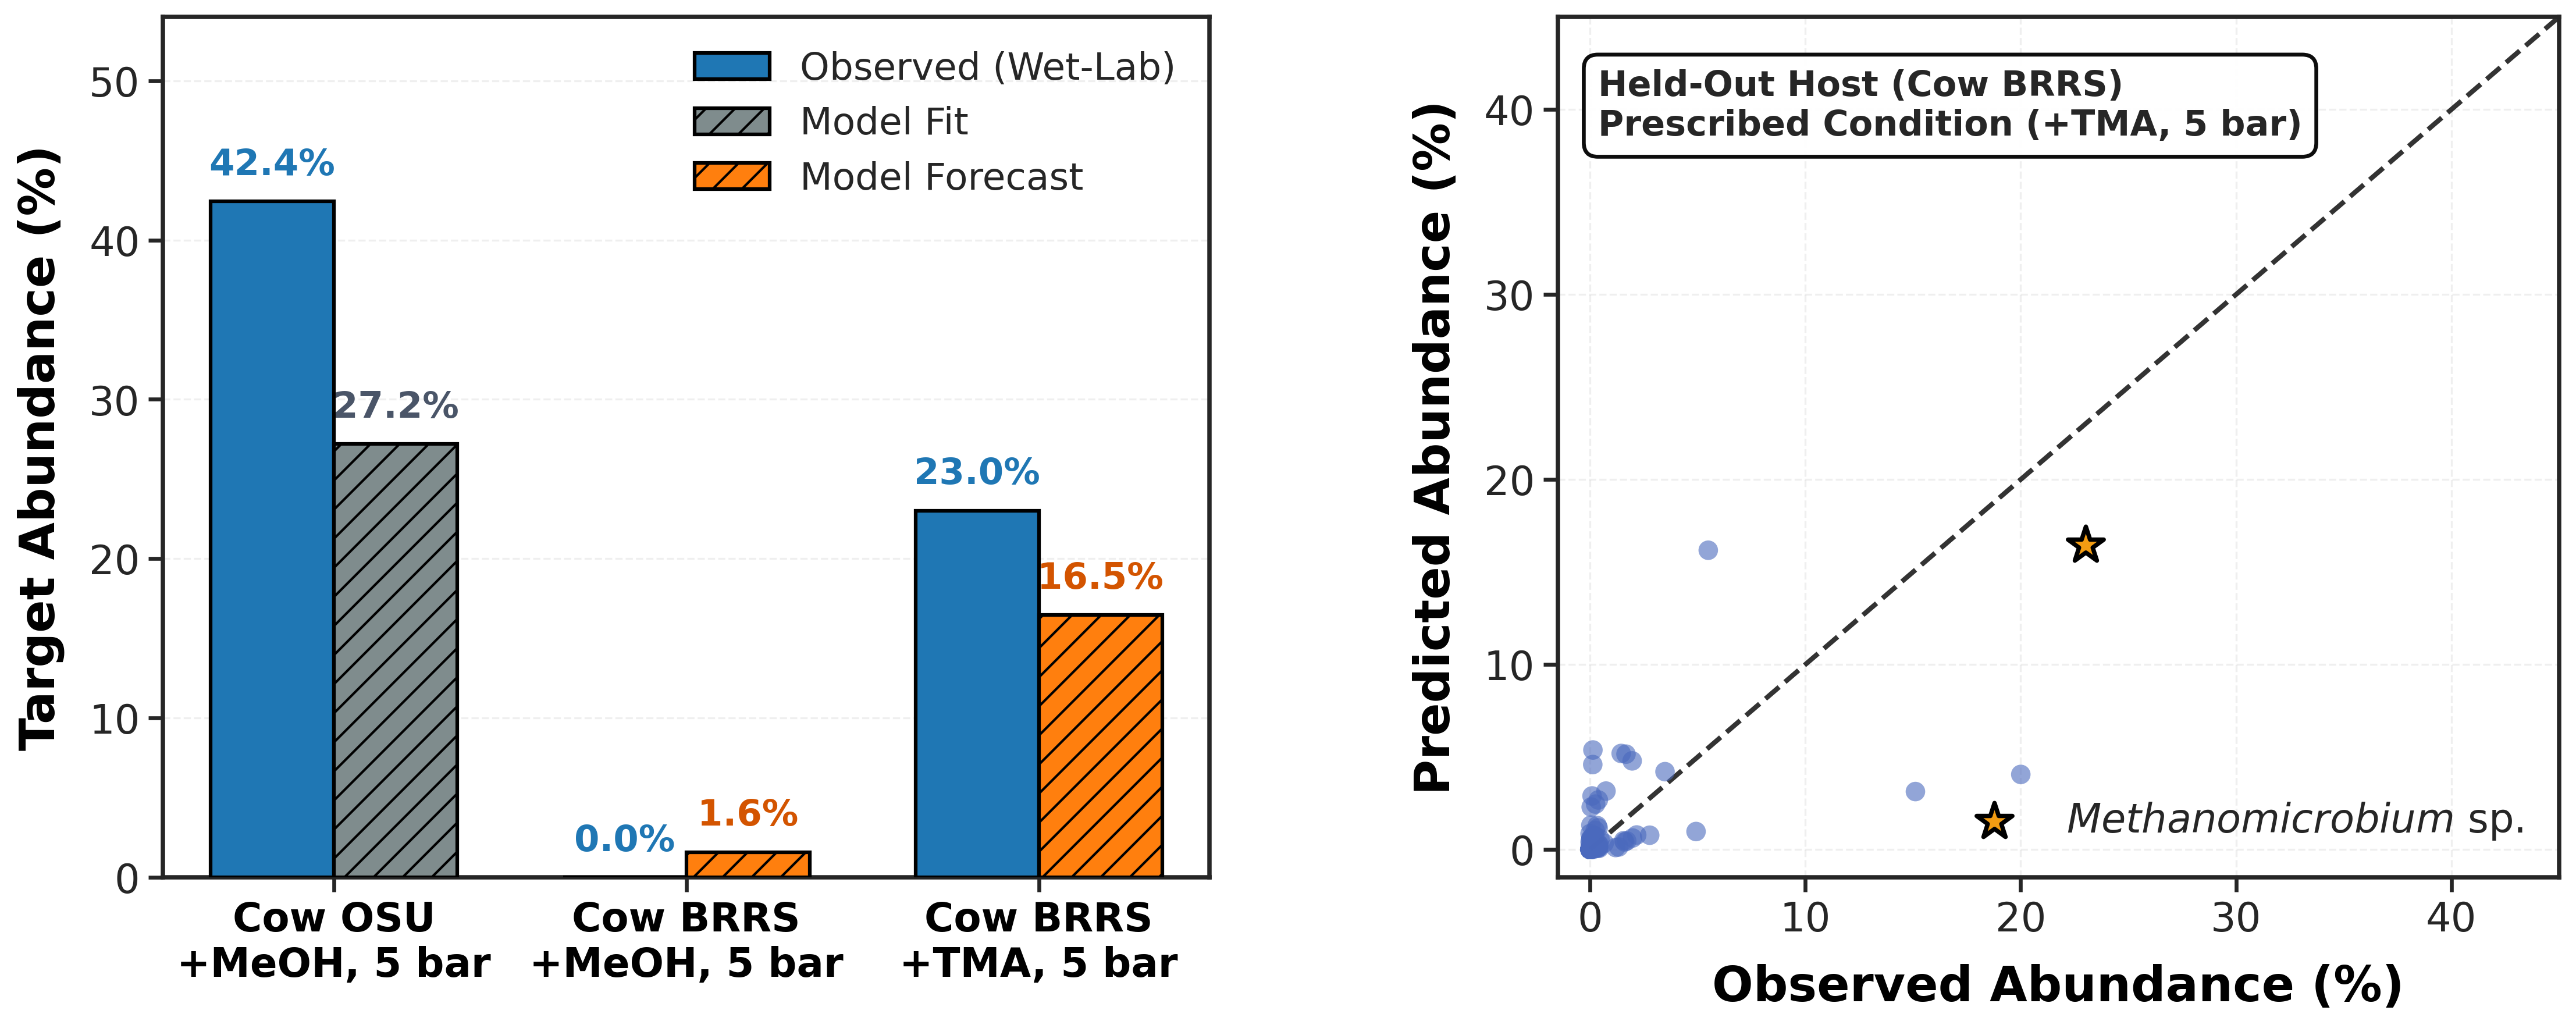
\includegraphics[width=0.88\linewidth]{figures/German_Prescriptive_Biotech_Search.png}
    \end{figure}
    \vspace{-1ex}
    \par{\scriptsize\textit{Data contributors:} Bela Haifa Khairunisa, Niel Baxter, Dwi Susanti, and Germ\'an Plata (BiomEdit Inc.); Christian Heryakusuma, Colin Short, and Biswarup Mukhopadhyay (Virginia Tech).}
  \end{block}



  % 7. GORE: MODEL FIT AND NON-EQUILIBRIUM OSCILLATIONS
  \begin{block}{Model provides mechanistic insight for cause of limit cycles}
    \begin{itemize}
      \item Synthetic bacterial consortia under daily serial dilution across low, medium, and high nutrient concentrations. Hu et al. (\textit{Science} 2022) explain stable vs.\ oscillatory behavior using medium-specific average interaction strengths.
      \item When species decouple resource \emph{uptake} from \emph{growth yield} ($\mathbf{\Phi}\neq\mathbf{\Theta}$), the effective interaction matrix $\mathbf{A} = \mathbf{\Theta}\tilde{\mathbf{R}}\mathbf{\Phi}^T$ becomes skew-symmetric, destroying MacArthur's Lyapunov function (Blumenthal et al., \textit{PRL} 2024) and enabling a supercritical Hopf bifurcation.
      \item Fitting the model to a high-fluctuation 3-species community with cyclic cross-feeding produces sustained limit cycles (ongoing work).
    \end{itemize}

    \begin{figure}
      \centering
      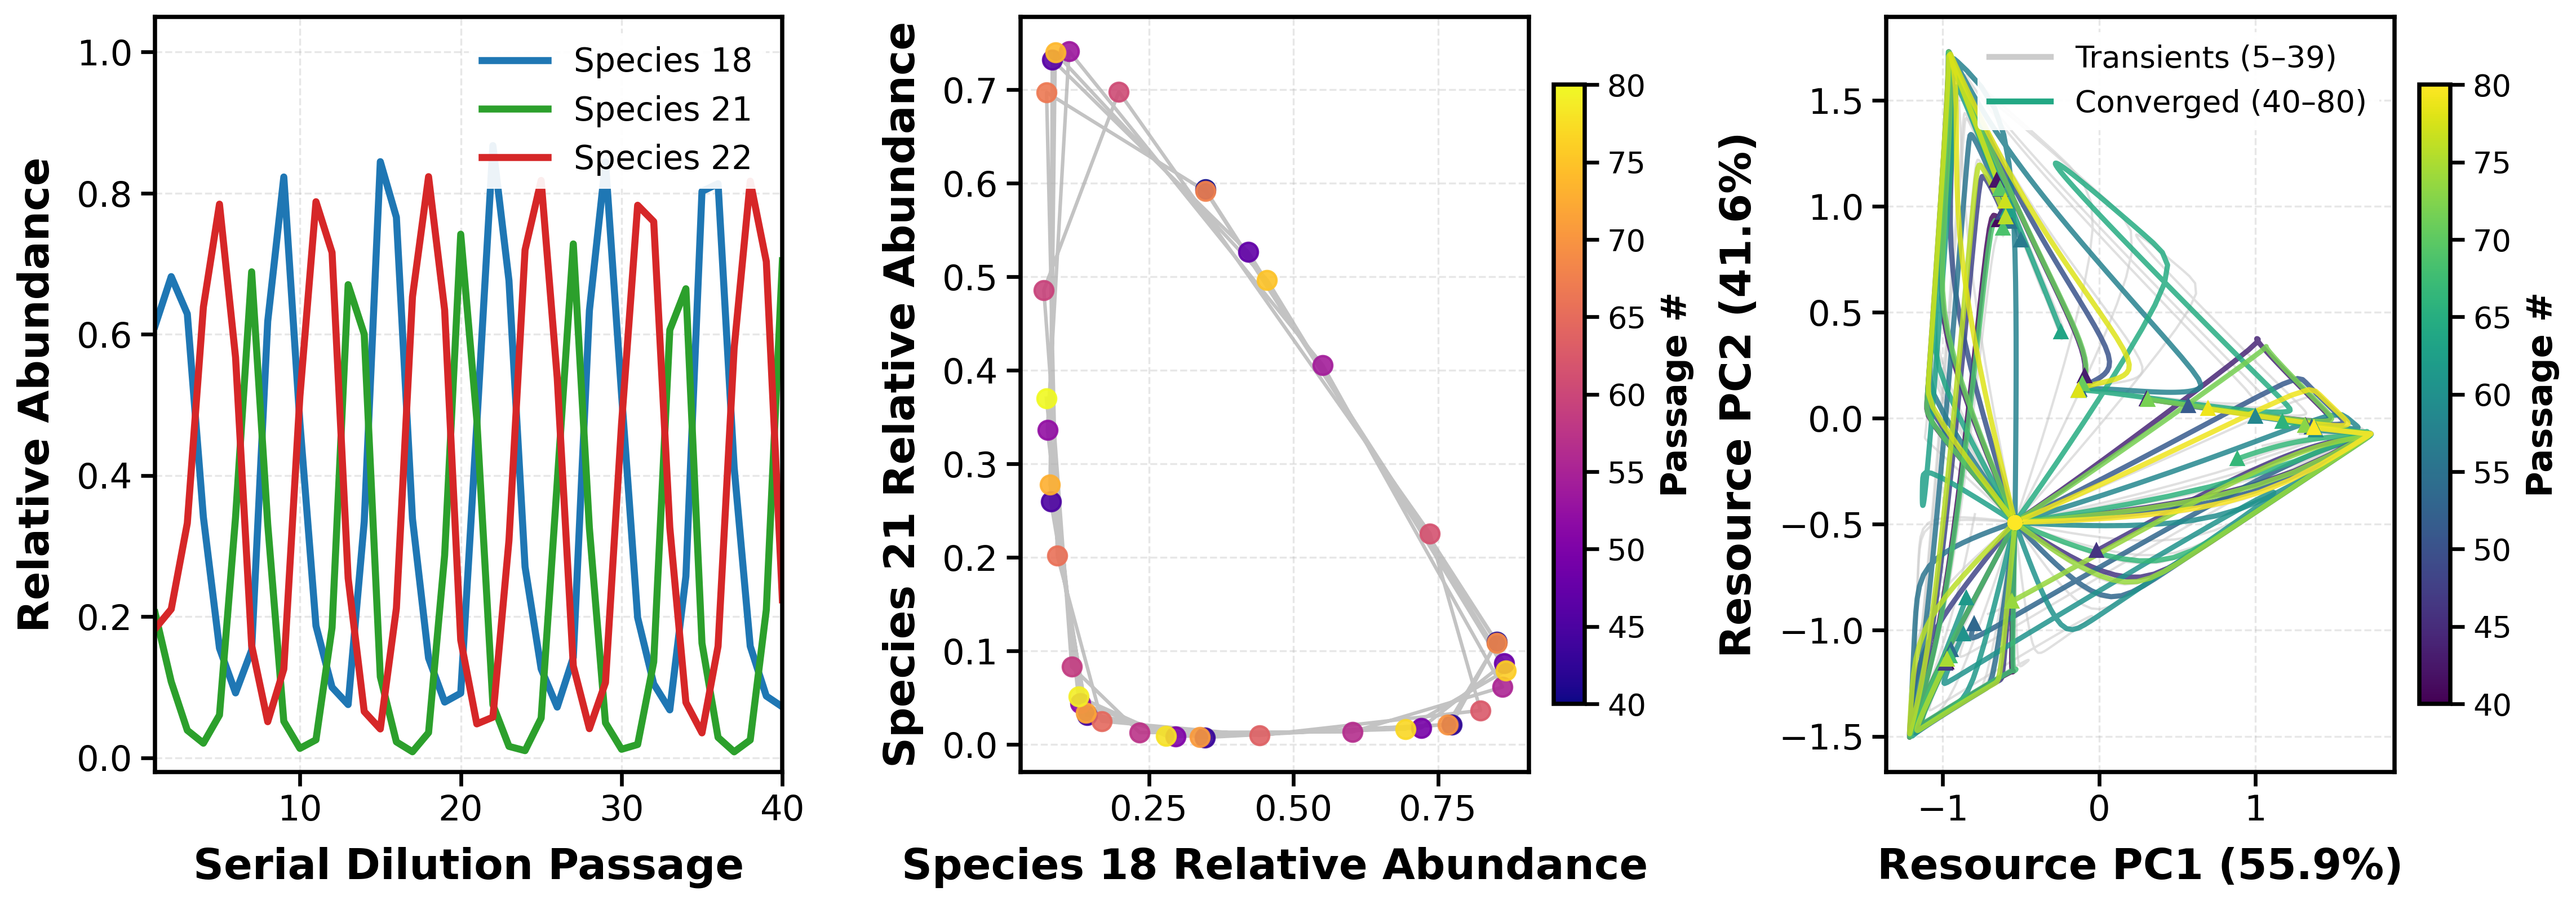
\includegraphics[width=0.94\linewidth]{figures/Gore_Oscillation_Combined_Panel.png}
    \end{figure}
  \end{block}

  % % 7. KEY TAKEAWAYS & CONCLUSIONS
  % \begin{block}{7. Key Takeaways \& Conclusions}
  %   \begin{enumerate}
  %     \item \textbf{Low-Dimensional Microbiomes:} Under serial dilution kinetics, high-dimensional CRMs collapse onto a $K \ll N$ latent resource manifold (Srinivasan et al., \textit{PRX Life} 2026), making community-level fitting tractable for the first time.
  %     \item \textbf{Trait Invariance:} Consumer-resource traits ($\mathbf{\Theta}, \mathbf{W}$) are transferable biological properties that generalize across spatial regimes, chemical additives, nutrient conditions, and community compositions.
  %     \item \textbf{Non-Equilibrium Bifurcations:} Environmental nutrient supply alone triggers transitions between stability and oscillation, mediated by the symmetry of growth vs.\ uptake ($\mathbf{\Phi}$ vs.\ $\mathbf{\Theta}$).
  %     \item \textbf{Predictive Bioengineering:} Learned traits support prescriptive media search, predicting conditions that rescue desired enrichment outcomes confirmed in wet lab.
  %   \end{enumerate}
  % \end{block}

  % REFERENCES
  \begin{block}{References}
    \footnotesize
    \begin{itemize}
      \setlength{\itemsep}{0pt}
      \item Srinivasan et al.\ \textit{PRX Life} \textbf{4}, 033026 (2026) --- Low-dimensional coexistence in complex microbial ecosystems.
      \item Blumenthal, Rocks \& Mehta. \textit{Phys.\ Rev.\ Lett.} \textbf{132}, 127401 (2024) --- Phase transition to chaos in complex ecosystems with nonreciprocal species-resource interactions.
      \item Hu et al.\ \textit{Science} \textbf{378}, 85--89 (2022) --- Emergent phases of ecological diversity and dynamics mapped in microcosms.
      \item Venturelli et al.\ \textit{Mol.\ Syst.\ Biol.} \textbf{14}, MSB178157 (2018) --- Deciphering microbial interactions in synthetic human gut microbiome communities.
      \item Jin et al.\ \textit{Nat.\ Commun.} \textbf{14}, 3510 (2023) --- Culturing of a complex gut microbial community in mucin-hydrogel carriers.
    \end{itemize}
  \end{block}

\end{column}

\separatorcolumn
\end{columns}
\end{frame}

\end{document}
